\chapter{Validação, benchmark e evidências complementares}
\label{app:validacao}

Este apêndice reúne os controles usados para auditar o cálculo marítimo e interpretar os benchmarks do \CabotageLens{}. Os números apresentados correspondem aos artefatos rastreados e permanecem vinculados à fonte, à unidade e à regra de agregação descritas no Capítulo~\ref{ch:validacao}.

\section{Fluxo de classificação da evidência}
\label{sec:app-mapa-validacao}

A Figura~\ref{fig:fluxo-classificacao-evidencia} mostra a passagem entre definição do cenário, execução, verificação da proveniência e classificação de uso. A disponibilidade de um resultado numérico não substitui a análise de sua fronteira.

\begin{figure}[htbp]
\centering
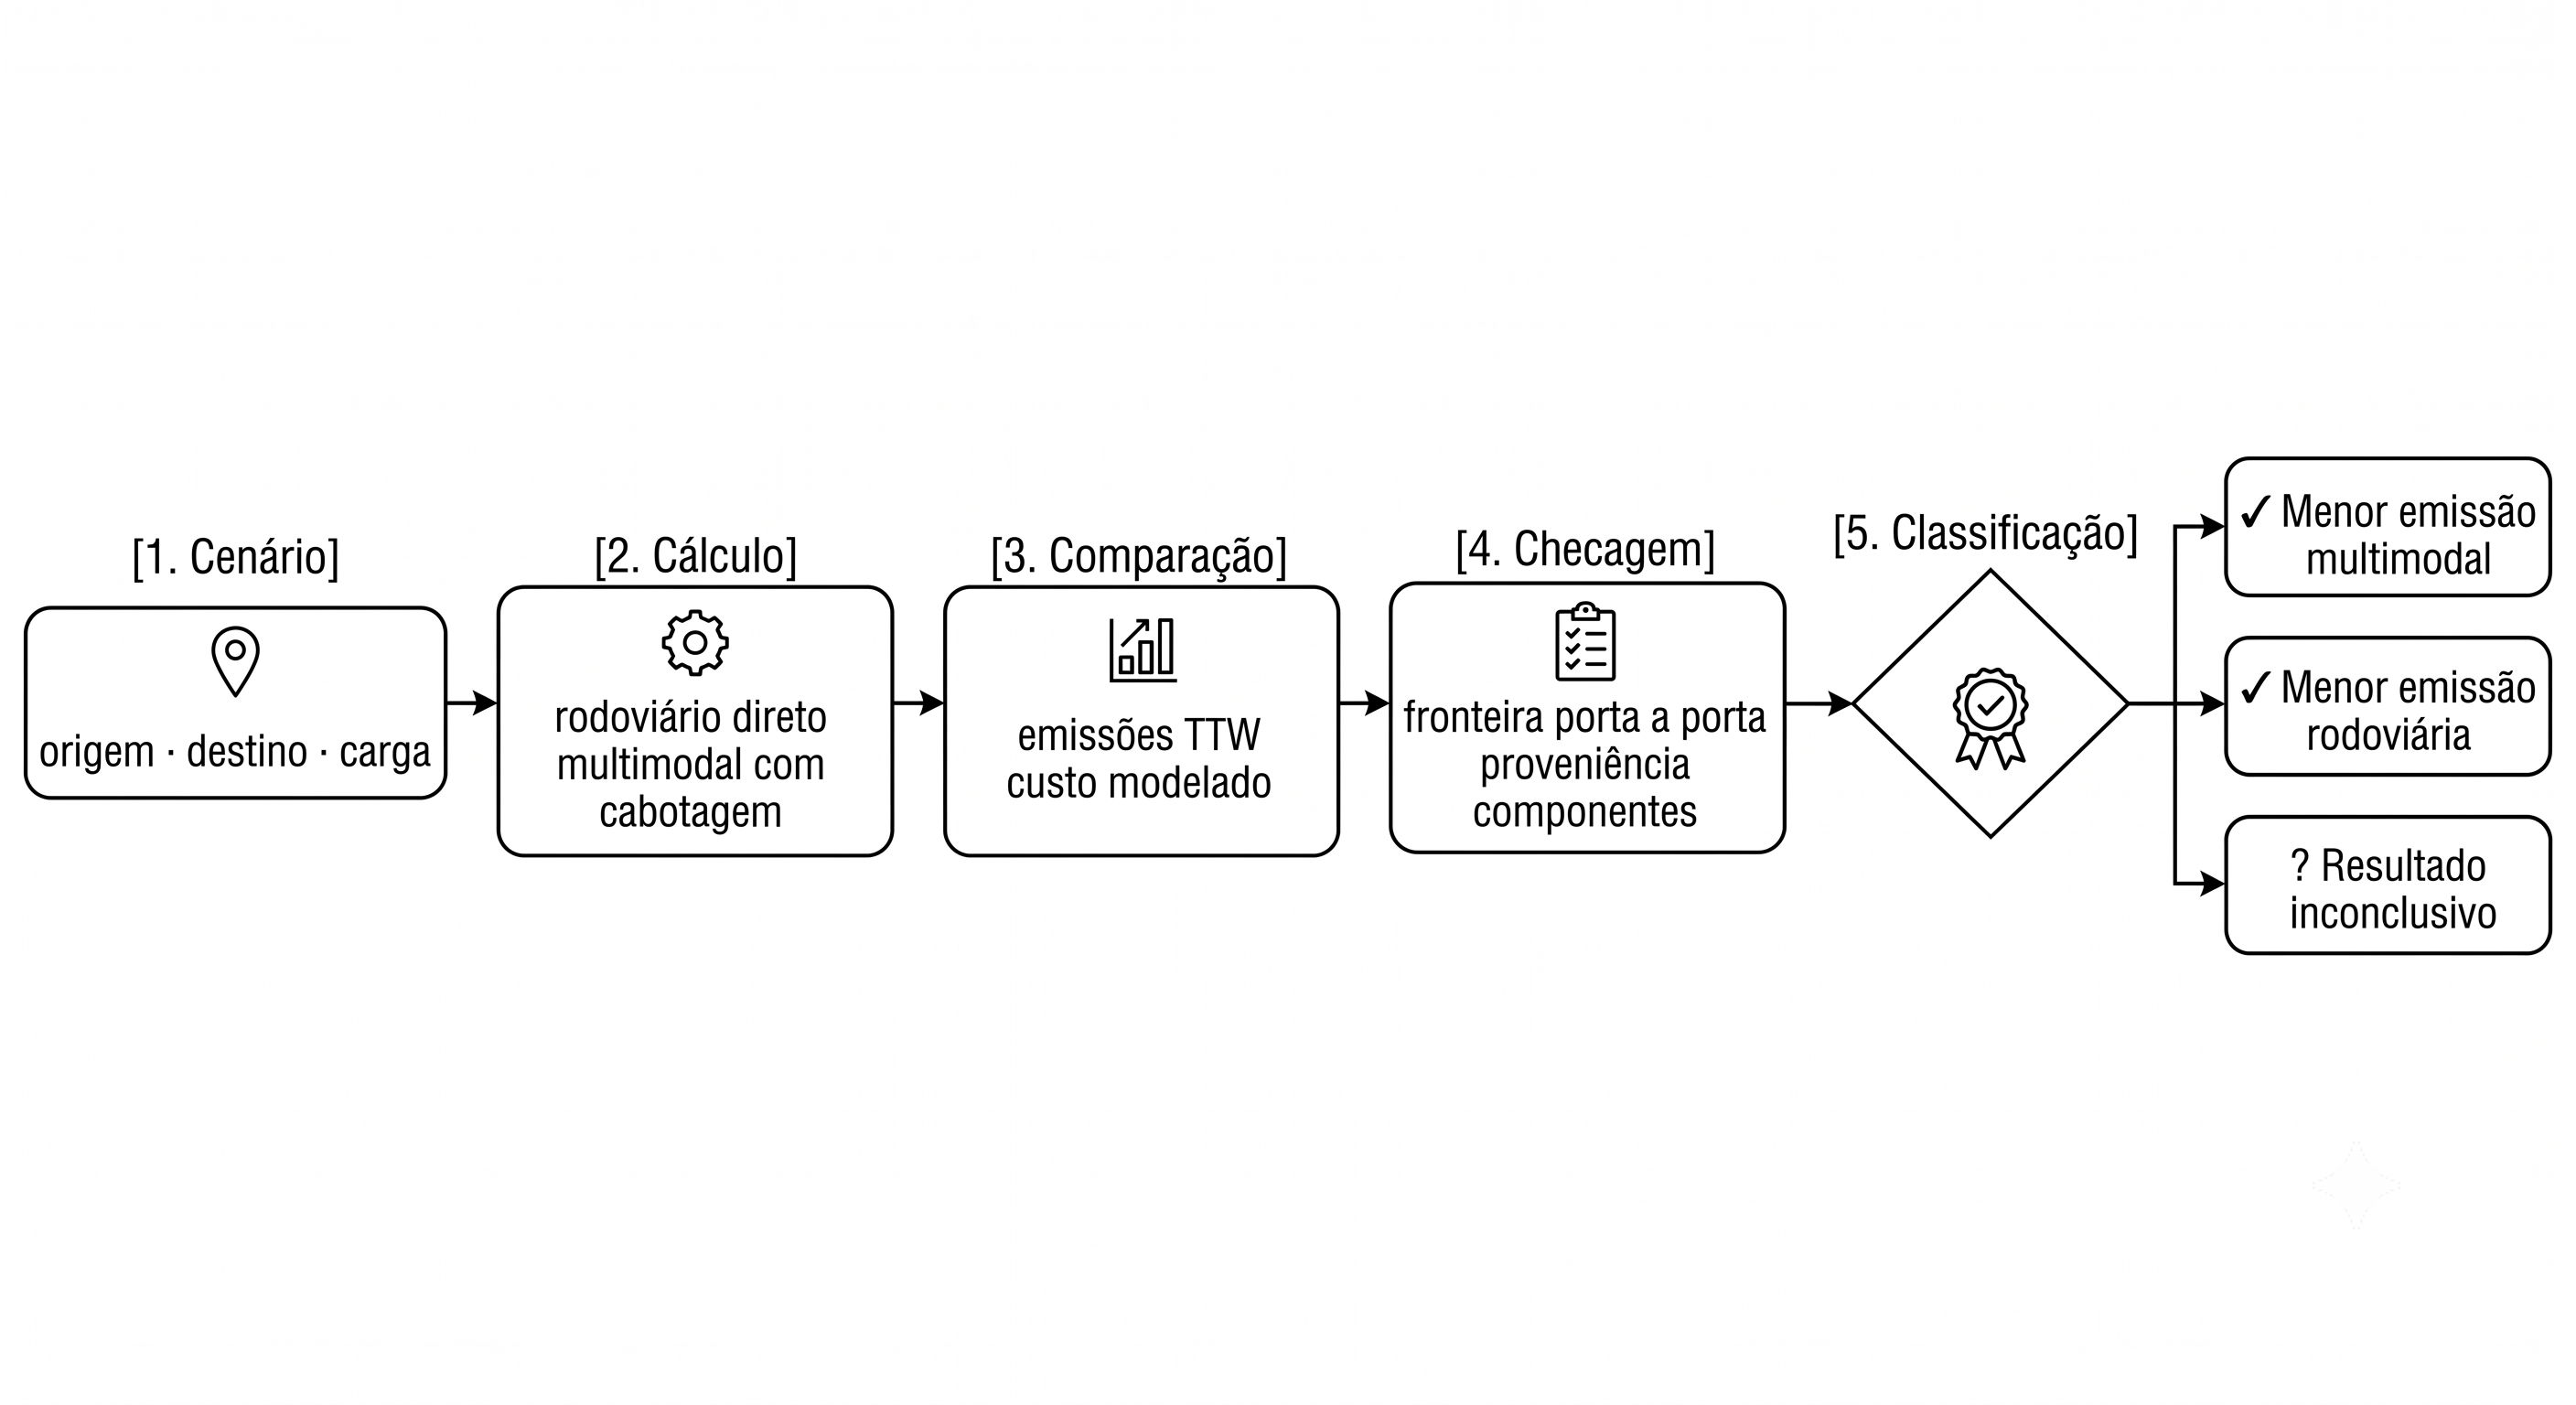
\includegraphics[width=0.95\textwidth]{images/figura_B_1.png}
\caption{Fluxo de classificação de evidências utilizado para organizar cada cenário avaliado.}
\label{fig:fluxo-classificacao-evidencia}
\end{figure}

\begin{table}[htbp]
\centering
\small
\caption{Perguntas de auditoria associadas às camadas de evidência.}
\label{tab:app-camadas-evidencia}
\begin{tabularx}{\textwidth}{L{0.26\textwidth}Y Y}
\toprule
Camada & Pergunta de auditoria & Registro esperado \\
\midrule
Dados ANTAQ & A sequência pertence à mesma viagem e a origem antecede o destino? & Identificador da viagem, ordem das escalas, movimentos de carga e cadeia completa de portos.\\
Intensidade MRV & O valor foi associado pelo IMO ou resolvido por fallback? & Fonte, ano, tipo ou classe, estatística robusta e tamanho da amostra.\\
Atividade da viagem & A carga a bordo e a distância foram aplicadas a cada subtrecho? & Massa, milhas náuticas, trabalho de transporte e combustível por subtrecho.\\
Agregação do par & Todas as viagens elegíveis contribuíram uma vez? & Contagens, pesos, mediana ponderada, regra de empate e tratamento de peso zero.\\
Geometria da rota & O caminho é uma sequência observada e contínua? & Portos, viagem candidata, critério de seleção e fontes de distância.\\
Resultado multimodal & As pernas usam a mesma unidade funcional e fronteira? & Carga do cenário, componentes rodoviários, marítimos e portuários, custo e emissões.\\
\bottomrule
\end{tabularx}
\end{table}

\section{Controles do artefato marítimo}
\label{sec:app-controles-artefato}

O arquivo direcional registra a versão de esquema, a data de geração, a hierarquia de intensidade, a política de outliers, o critério de seleção de corredor e os contadores de cobertura. A Tabela~\ref{tab:app-controles-artefato} consolida os campos que permitem rejeitar um artefato incompleto ou interpretar sua composição.

\begin{table}[htbp]
\centering
\footnotesize
\setlength{\tabcolsep}{4pt}
\renewcommand{\arraystretch}{1.15}
\caption{Controles de proveniência da matriz marítima direcional.}
\label{tab:app-controles-artefato}
\begin{tabularx}{\textwidth}{L{0.29\textwidth}L{0.27\textwidth}Y}
\toprule
Controle & Valor registrado & Função \\
\midrule
Esquema de intensidade & \codecell{maritime\_intensity\_schema\_version = 3} & Identifica a estrutura compatível com agregação por viagem--OD.\\
Modo de observação & \codecell{observed\_voyage\_corridors} & Restringe os caminhos a sequências completas de uma mesma viagem.\\
Escopo da intensidade & Todas as viagens elegíveis do mesmo par, em todos os corredores. & Define a população usada no estimador.\\
Estimador & Mediana ponderada por t$\cdot$nm. & Reduz a influência de intensidades extremas e preserva a atividade observada como peso.\\
Seleção do caminho & Ligação direta primeiro; depois, menor distância completa. & Separa geometria de rota e agregação estatística.\\
Reconstrução da carga & Deslocamento mínimo não negativo do prefixo acumulado. & Impede carga a bordo negativa e preserva movimentos observados.\\
Fallback de distância & Haversine para portos canônicos distintos sem valor positivo na matriz. & Mantém completude com fonte identificada.\\
Fallback de intensidade & Tipo com média aparada em 1\% por cauda ou mediana quando o corte não é possível; classe com média aparada do artefato ou mediana quando indisponível. & Explicita a estatística e a política de outliers.\\
\bottomrule
\end{tabularx}
\end{table}

\begin{table}[htbp]
\centering
\small
\caption{Contadores de cobertura preservados no artefato marítimo.}
\label{tab:app-contadores-maritimos}
\begin{tabularx}{\textwidth}{Y r Y}
\toprule
Contador & Valor & Observação \\
\midrule
Viagens / paradas / chamadas portuárias & \num{1324} / \num{6797} / \num{7103} & Estrutura observacional da ANTAQ.\\
IMOs ANTAQ / IMOs associados ao MRV & \num{389} / \num{243} & Cobertura de intensidade específica.\\
Subtrechos brutos / calculados & \num{5473} / \num{5438} & Diferença explicada por aliases consecutivos contraídos.\\
Distância da matriz / haversine & \num{5023} / \num{415} & Proveniência da distância por subtrecho.\\
Intensidade IMO / fallback & \num{3290} / \num{2148} & Proveniência da intensidade por subtrecho.\\
Observações viagem--OD / pares direcionados & \num{12025} / \num{177} & Base da agregação por origem--destino.\\
\bottomrule
\end{tabularx}
\end{table}

\section{Exemplo completo de auditoria: Santos--Manaus}
\label{sec:app-santos-manaus}

Para Santos--Manaus, a população estatística reúne \num{89} observações viagem--OD distribuídas em \num{22} corredores. Cada observação soma todos os seus subtrechos entre os dois portos e contribui uma única vez para a distribuição do par. A Tabela~\ref{tab:app-santos-manaus} permite conferir a separação entre a intensidade representativa e o caminho utilizado no cenário.

\begin{table}[htbp]
\centering
\small
\caption{Proveniência do par Porto de Santos--Porto de Manaus.}
\label{tab:app-santos-manaus}
\begin{tabularx}{\textwidth}{L{0.37\textwidth}Y}
\toprule
Campo & Valor \\
\midrule
Viagens resolvidas com trabalho positivo & \num{89} \\
Corredores completos observados & \num{22} \\
Observações com IMO exato & \num{40} \\
Observações com fallback de tipo & \num{49} \\
Participação do fallback no trabalho de transporte & \num{59.54}\% \\
Intensidade representativa & \num{9.322050} g/(t$\cdot$nm) \\
Método & Mediana inferior ponderada pelo trabalho de transporte \\
Caminho selecionado & Porto de Santos--Porto de Manaus \\
Critério do caminho & Ligação direta observada \\
Distância selecionada & \num{6112} km \\
\bottomrule
\end{tabularx}
\end{table}

A presença de uma ligação direta determina apenas o caminho. As viagens que passam por Itajaí, Paranaguá, Salvador, Suape, Pecém, Vila do Conde e outros portos permanecem na população estatística quando formam uma cadeia completa em que Santos antecede Manaus. O cálculo utiliza, portanto, a diversidade observada de corredores sem impor uma sequência portuária única.

\section{Fronteira de operações portuárias e \emph{hoteling}}
\label{sec:app-nota-portops-hoteling}

Quando o consumo marítimo é calculado com a intensidade MRV por trabalho de transporte, o indicador anual é tratado como abrangente do consumo reportado da embarcação para a fronteira considerada. O \emph{hoteling} não é somado separadamente nesse modo, reduzindo o risco de dupla contagem. As operações portuárias permanecem componentes explícitos quando possuem fonte identificada. Valores observados, médias de portos observados, padrões documentados e indisponibilidade são categorias distintas de proveniência; uma ausência não é convertida em zero de atividade.

\section{Benchmark externo}
\label{sec:app-benchmark}

\begin{table}[htbp]
\centering
\small
\caption{Resumo do benchmark externo associado aos estudos de Gustavo Costa.}
\label{tab:app-benchmark-resumo}
\begin{tabularx}{\textwidth}{L{0.40\textwidth}r Y}
\toprule
Item & Valor & Interpretação \\
\midrule
Células de matriz parseadas & \num{36} & Inventário total lido pelo roteiro de comparação.\\
Pares positivos e suportados & \num{21} & Denominador da comparação direcional.\\
Pares não comparáveis & \num{15} & Seis pares iguais e nove linhas rodoviárias nulas ou não positivas.\\
Acordo direcional & 21/21 & As duas fontes favorecem a alternativa com cabotagem em emissões.\\
Classificação & \codecell{same\_direction\_large\_gap} & Apoio ao sinal modal, sem equivalência de magnitude.\\
\bottomrule
\end{tabularx}
\end{table}

A comparação preserva as diferenças de distância, carga, portos, alocação, fatores e fronteira ambiental. Seus parâmetros permanecem separados dos parâmetros operacionais do aplicativo; o benchmark apoia a leitura do sinal modal, mas não calibra a intensidade marítima nem a magnitude dos resultados.

\section{Categorias de uso}
\label{sec:app-categorias-uso}

A Tabela~\ref{tab:app-categorias-uso} resume as categorias utilizadas para controlar afirmações. Ela complementa a Tabela~\ref{tab:categorias-uso}.

\begin{table}[htbp]
\centering
\footnotesize
\setlength{\tabcolsep}{4pt}
\renewcommand{\arraystretch}{1.15}
\caption{Resumo operacional das categorias de evidência.}
\label{tab:app-categorias-uso}
\begin{tabularx}{\textwidth}{L{0.35\textwidth}Y}
\toprule
Categoria & Leitura permitida \\
\midrule
\codecell{headline\_candidate} & Resultado principal somente com rota, fonte, unidade e fronteira suficientes.\\
\codecell{sensitivity\_discussion} & Comportamento condicionado à premissa identificada.\\
\codecell{limitation\_example} / \codecell{excluded} & Exemplo de limite ou cenário fora da fronteira de uso.\\
\codecell{reference\_needed} / \codecell{methodology\_blocked} & Lacuna de fonte ou de decisão que impede conclusão quantitativa.\\
\codecell{benchmark\_supports\_direction} & Consistência direcional sem calibração de magnitude.\\
\codecell{benchmark\_boundary\_mismatch} / \codecell{not\_comparable} & Diferença de fronteira ou ausência de comparabilidade numérica.\\
\bottomrule
\end{tabularx}
\end{table}
